%
% Webapplikation
% Abschlussarbeit (Bachelor)
%
% Thema: Erstellung einer Browser Extension zur Usability Evaluierung von beliebigen Web-Applikationen über Heatmaps.
% Betreuer 1: Prof. Dr. Targo Pavlista
% Betreuer 2: Siamak Haschemi
%
% @author Christian Bromann <contact@christian-bromann.com>
%

\section{Webapplikation}

Die Webapplikation ist die Administrationsoberfläche der gesamten Anwendung. Hier erstellt der User des \textit{thEvaluator} Frameworks die Testcases, passt sie an und wertet sie anschließend aus. Wie es sich für einen administrativen Bereich gehört, sollte dieser passwortgeschützt sein und nur bestimmten Personen Zugang gewähren. Aus zeitlichen Gründen wurde jedoch auf ein User-Management verzichtet. Betritt man die Startseite des Bereiches, so erhält der User eine Übersicht über die bereits angelegten Testcases. Neben dem Namen sind drei Aktionsbuttons zu finden, mit denen man den Testcase bearbeiten, löschen oder dessen Details betrachten kann. Ganz oben neben dem \textit{thEvaluator} Logo befindet sich die Navigation. Diese leitet den Benutzer zum Erstellen oder Evaluieren von Testcases weiter.

\begin{center}
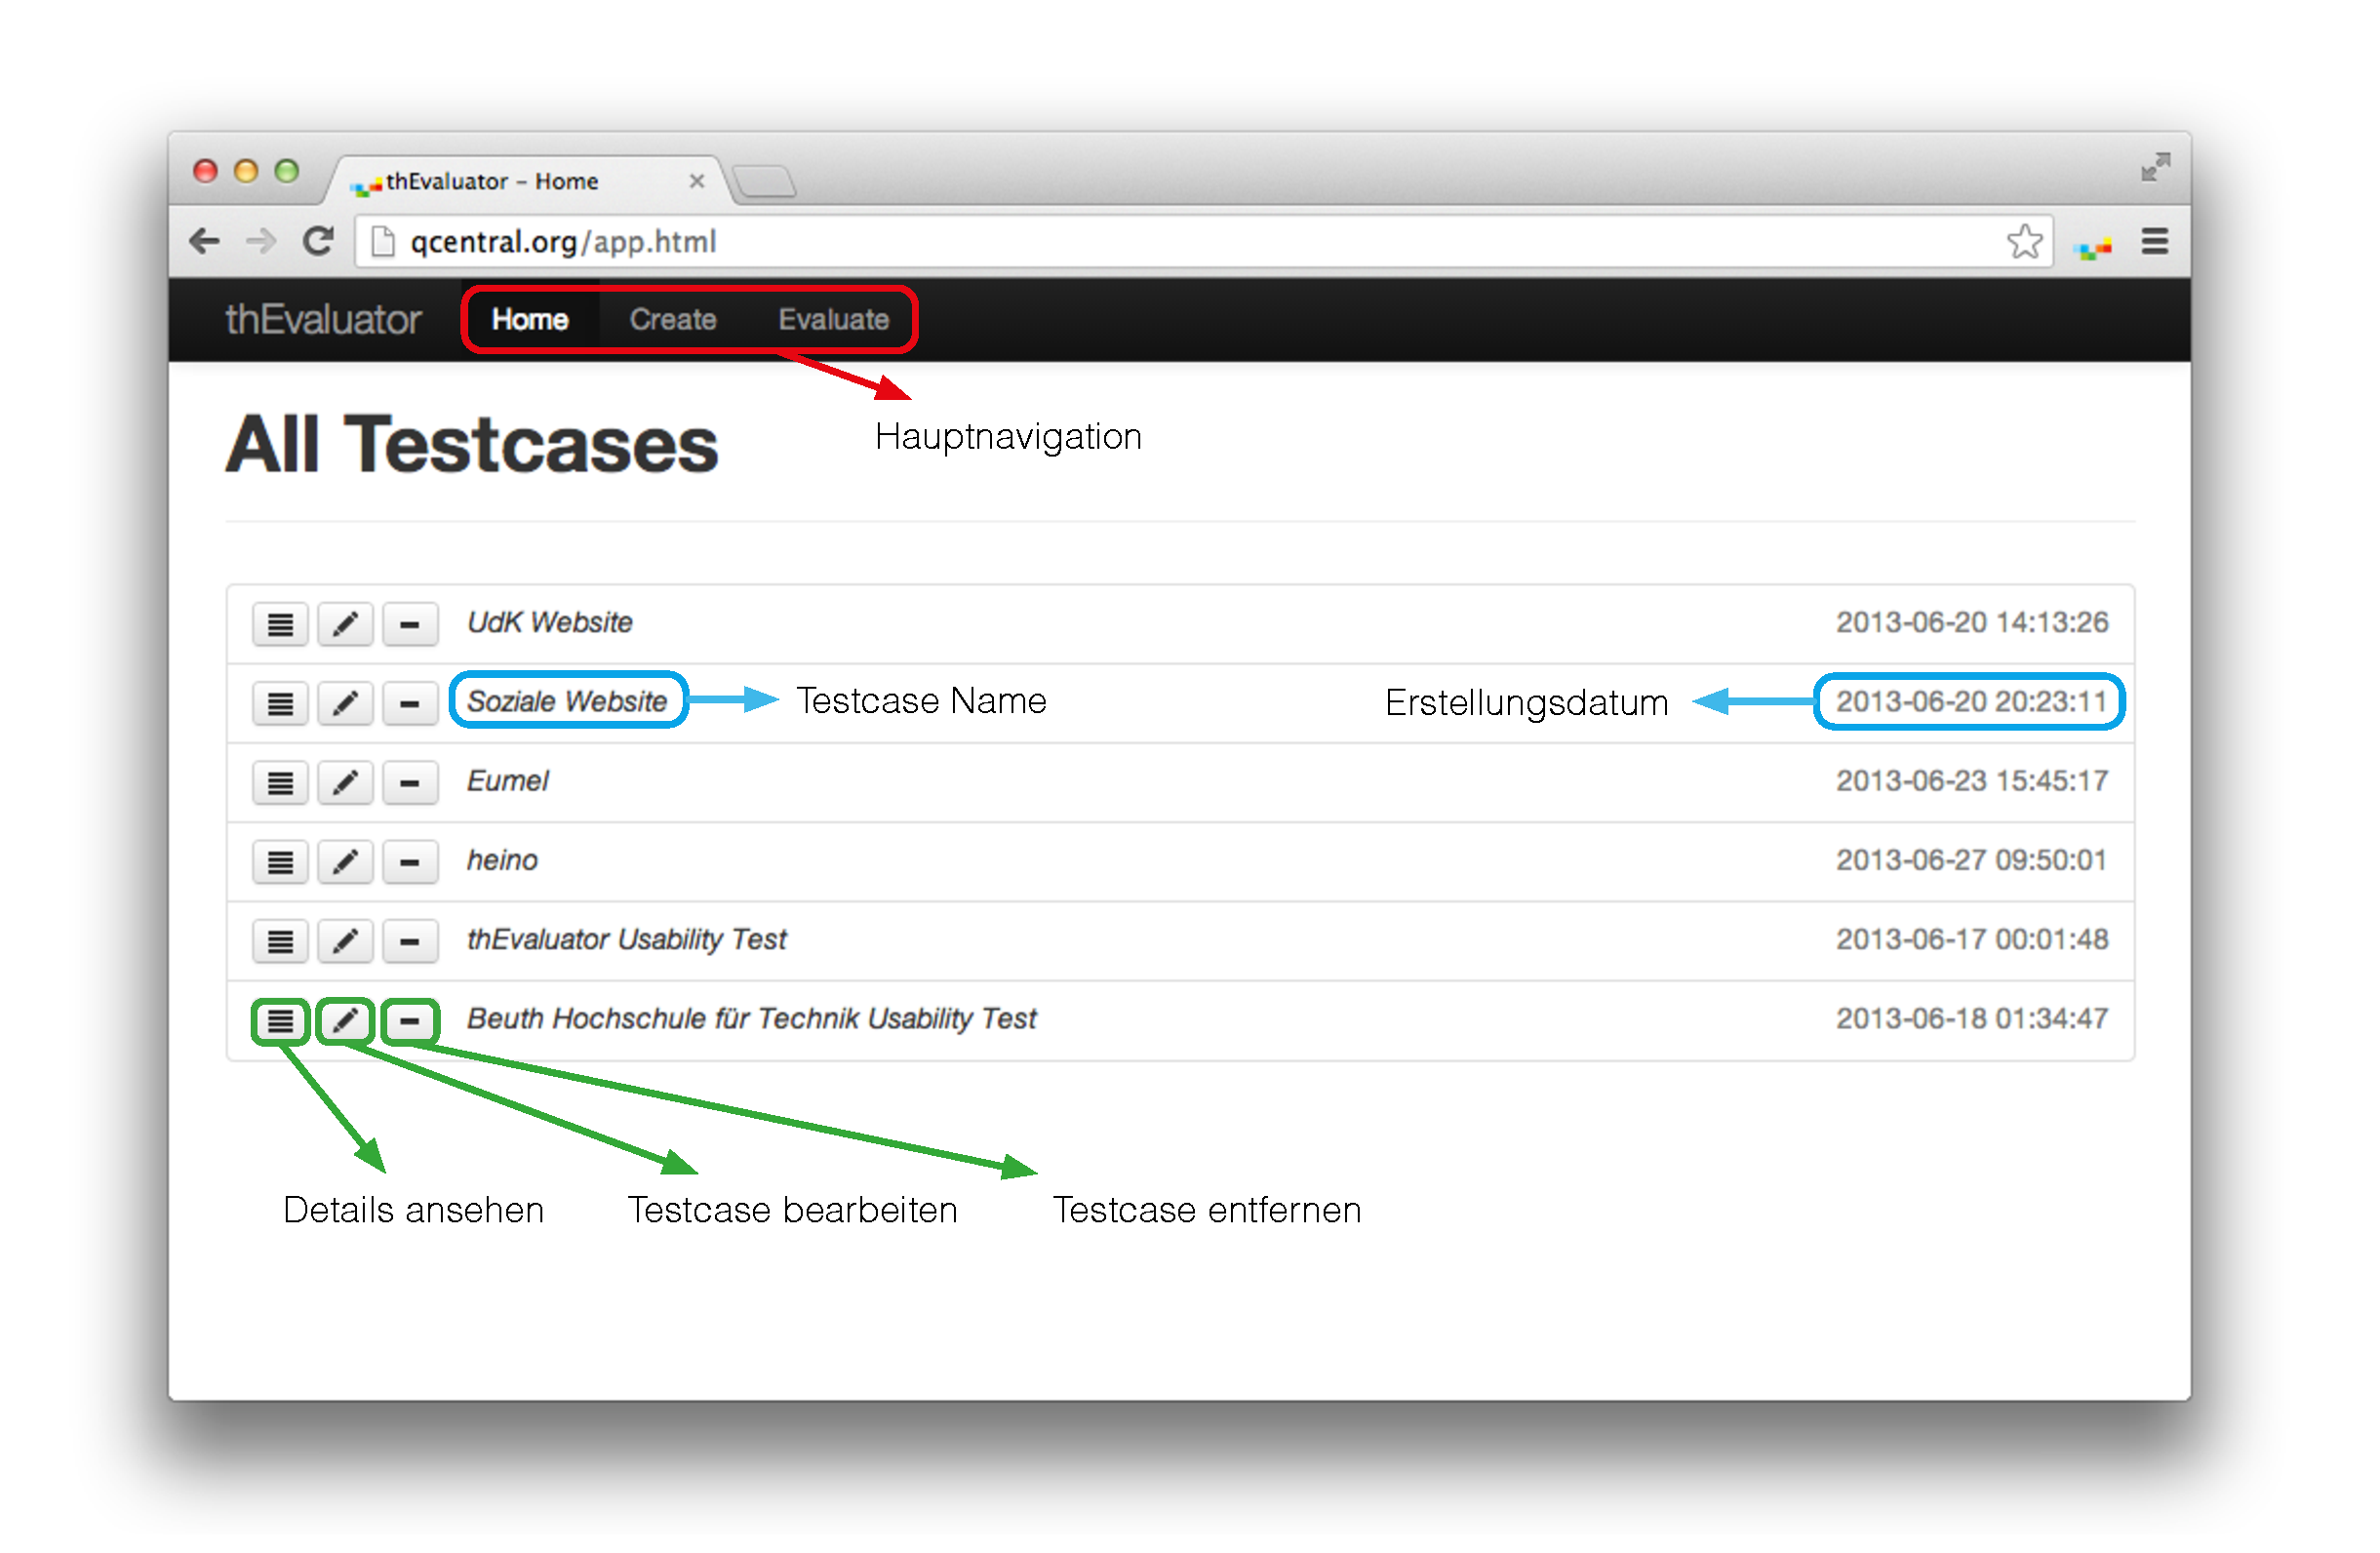
\includegraphics[scale=0.40]{./images/webappscreen}
\end{center}
\begin{figure}[htb]
   \centering
   \caption{Administrationsoberfläche}
    \label{webappview}
\end{figure}

Alles beginnt mit der Erstellung eines Testcases. Es braucht nicht viel Zeit und Eingaben, um einen zu erstellen. Nach dem Klick auf \textit{Create} öffnet sich die Formularansicht. Als erstes vergibt man einen Namen für den Testcase, gefolgt von einer URL. Diese ist der Startpunkt für den Testcase. Es ist dabei nicht notwendig von der Startseite einer Website zu beginnen. Führt man bspw. einen Test für das firmeninterne Intranet durch, so kann auch eine Netzwerk-URL eingegeben werden. Wichtig ist nur, dass die Teilnehmer die notwendigen Rechte zum Zugriff auf die Seite besitzen. Eine weitere wichtige Angabe ist die der Auflösung. Jeder Testcase muss eine feste Auflösung vorschreiben, um die Verhältnisse für jeden Probanden gleich zu setzen. Die Extension verkleinert oder vergrößert beim Starten des Testcases dann automatisch das Browserfenster. Dadurch wird sichergestellt, dass die Testuser unter den gleichen Vorraussetzungen, was Auflösung angeht, die Seite nutzen. Zudem ermöglicht es Usability-Tests für Webseiten mit einem \textit{Responsive Design}. Wählt der User eine Auflösung für mobile Geräte, wie z.B. 320 x 480 px, so erhält er automatisch die Version der Website, die ein mobiler User ebenfalls erhalten würde. Obwohl das Verhalten zwischen Mobil- und Desktop-User dann immer noch nicht das Gleiche ist, bekommt man trotzdem einen recht guten Eindruck davon, wie die mobile Version der Seite genutzt wird.

\begin{center}
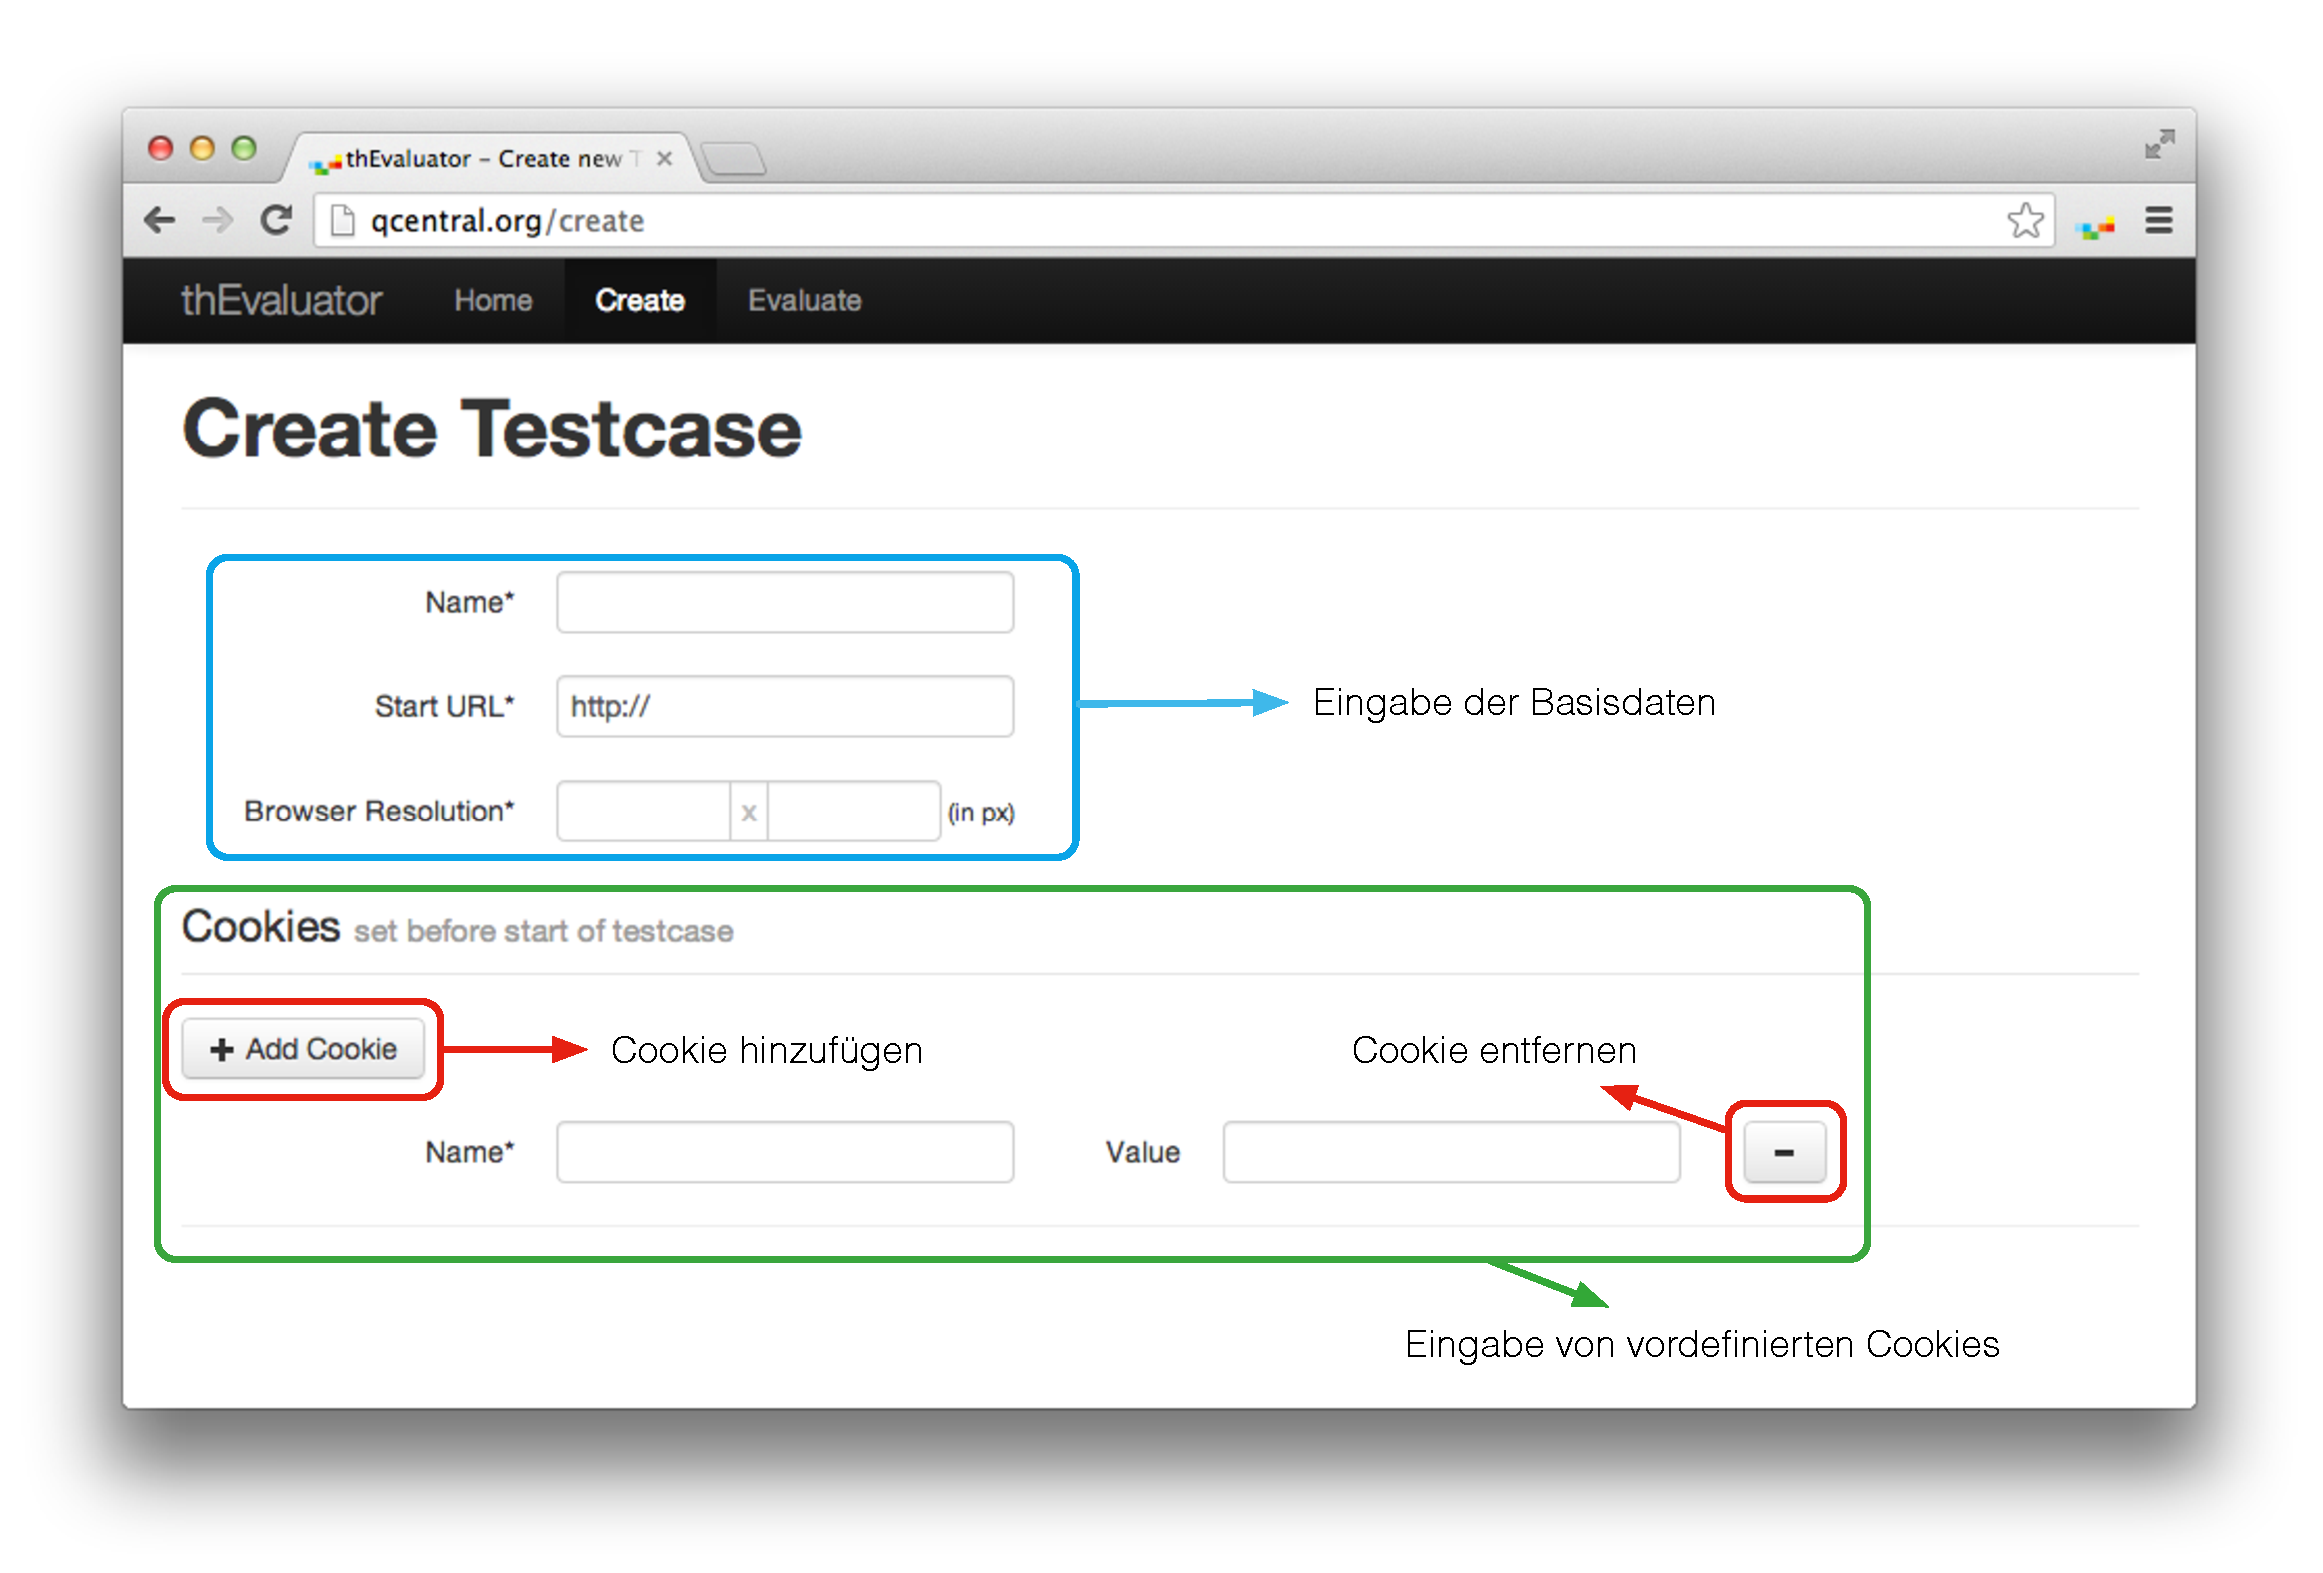
\includegraphics[scale=0.40]{./images/createscreen}
\end{center}
\begin{figure}[htb]
   \centering
   \caption{Formularansicht}
    \label{createview}
\end{figure}

Um den Usability-Test für jeden Bereich einer Webseite möglich zu machen, gibt es zudem die Möglichkeit, Cookies vor dem Start setzen zu lassen. Möchte der User bspw. eine Website testen lassen, die noch nicht veröffentlicht ist, so kann er hier spezielle Cookies definieren, die die Seite erkennt und den Zutritt darauf gewährt. Die Extension setzt diese Cookies vor Beginn des Testcases für alle Subdomains und Pfade der Website. Als letztes werden die Tasks definiert. Diese enthalten, neben dem Namen und einer Aufgabenbeschreibung, ein \textit{required} Feld, welches angibt, ob der Testcase beendet ist, wenn der Proband die Aufgabe nicht lösen kann. Dadurch ist es möglich, eine Aufgabe, wie z.B. die Auswahl eines Produktes im Online-Shop, als Vorraussetzung für die Folgeaufgaben, z.B. die Ware in den Warenkorb zu packen, auszuwählen.

\begin{center}
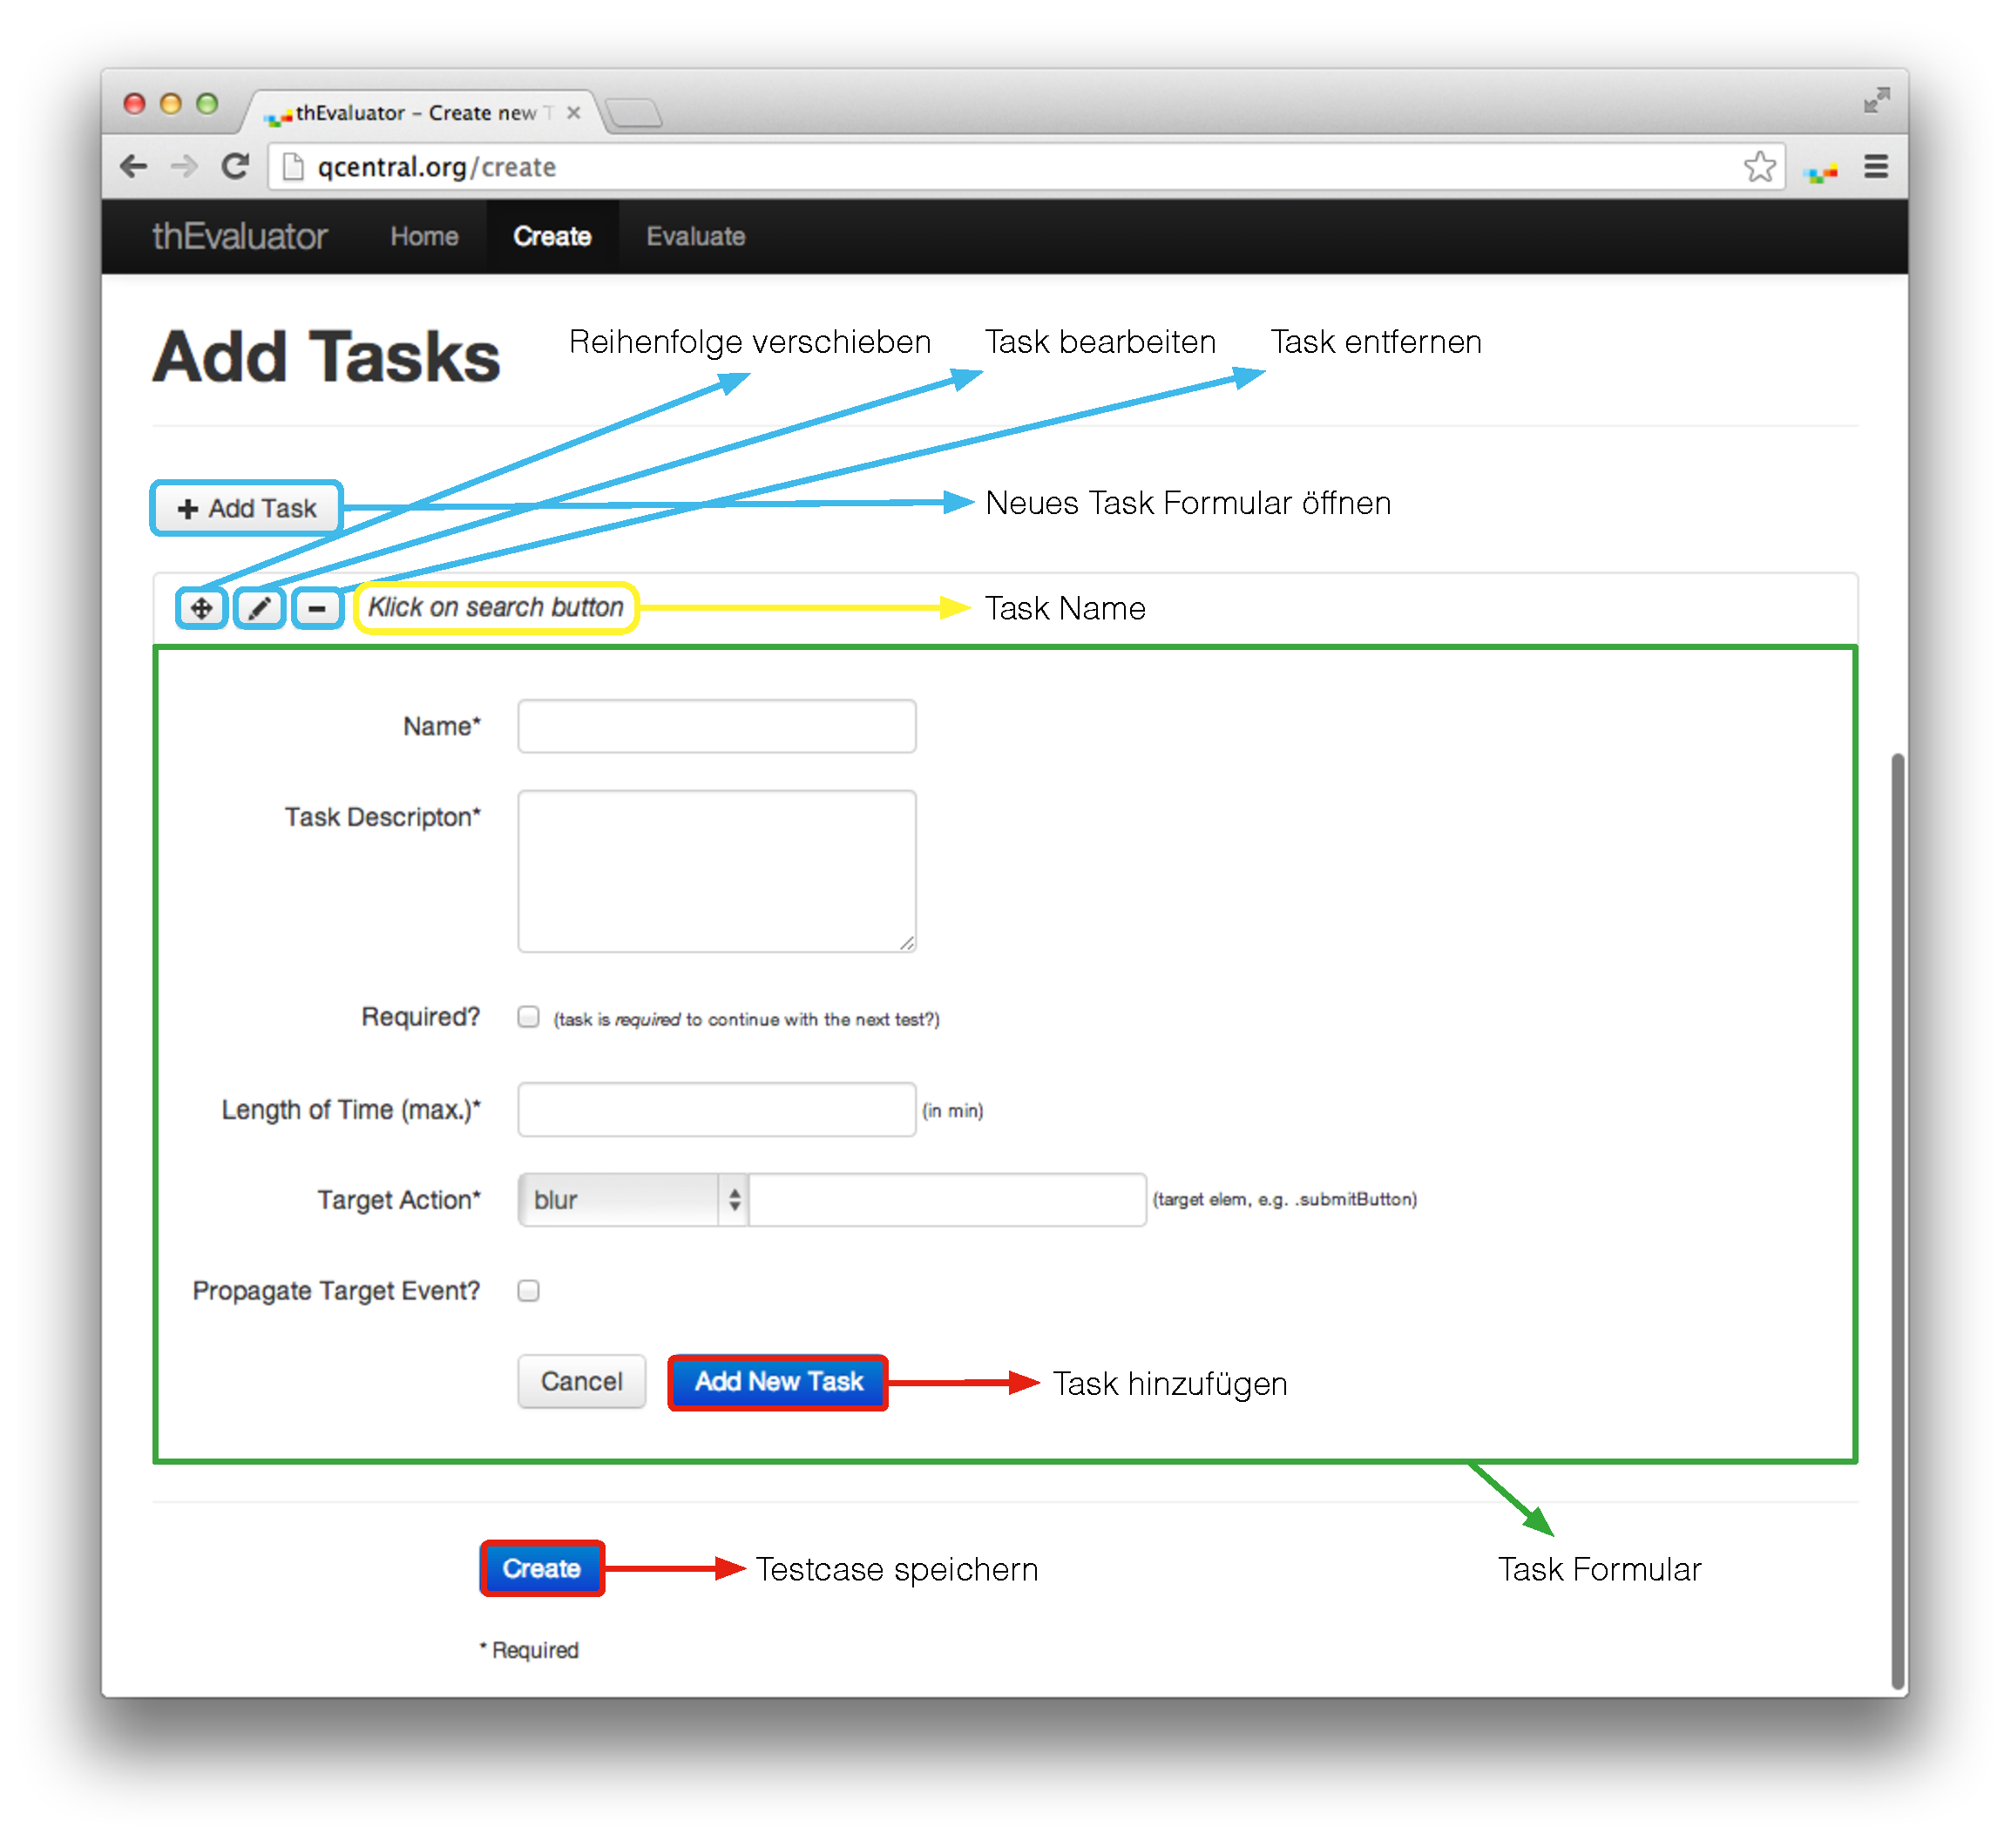
\includegraphics[scale=0.4]{./images/taskscreen}
\end{center}
\begin{figure}[htb]
   \centering
   \caption{Task-Formular}
    \label{taskscreen}
\end{figure}

\label{targetElem}
Ein weiteres Attribut eines Tasks ist die Zeit. Die Aufgabe kann als gescheitert angesehen werden, wenn der Proband zu lange zum Lösen dieser benötigt. In einem realen Szenario würde der User eine Website verlassen, wenn er nach einer bestimmten Zeit nicht an sein Ziel findet. Als nächstes folgt die Angabe des Ziel Events. Dieses besteht, wie in Kapitel \ref{events} beschrieben, besteht dieses aus einer Action und einem Element aus dem DOM. Möchte man bspw. den Klick auf einem Link mit einer bestimmten URL als Ziel einer Aufgabe definieren, so wählt man eine \textit{click}-Action auf einem Element mit dem Selektor \textit{a[href=''\textbf{ URL }'']}. Es kann auf alle CSS3 Selektoren zurückgegriffen werden. Dies macht die Einschränkung der Elemente sehr flexibel. Als letztes ist die Angabe des \textit{Propagation} Attributes möglich. Dies setzt fest, ob das Event, wie z.B. der Klick nach dem Abfangen durch die Extension abgefangen werden soll oder nicht. Bleiben wir beim Beispiel mit dem Klick auf einen Link, so würde sich die neue Seite nur öffnen, wenn die Checkbox aktiviert ist. Der User würde dann mit dem nächsten Task auf dieser Seite weiter machen. Ist die Box nicht aktiviert, so verbleibt er auf der Seite, da die Extension den Klick abfängt, bevor der Browser den Befehl zum Öffnen der neuen Seite bekommt.\\
\\
Nachdem ein paar Aufgaben für den Testcase erstellt wurden, ist im Nachhinein noch möglich, jeden einzelnen Task zu bearbeiten. Zudem kann die Reihenfolge der Aufgaben via Drag\&Drop verschoben werden (siehe \glqq Reihenfolge verschieben\grqq{}-Button in Abbildung \ref{taskscreen}). Als letztes wird der Testcase gespeichert und erhält eine 10-stellige ID, die allen Probanden geschickt werden kann, die an dem Test teilnehmen. Zum Schluss können die Ergebnisse auf der \textit{Evaluate} Seite (siehe Hauptnavigation) ausgewertet. Näheres dazu wird in Kapitel \ref{evaluation} erläutert.


\subsection{Deployment}

Die Webapplikation des \textit{thEvaluator} Frameworks ist mit den modernsten Frontend-Web-Technologien dieser Zeit entwickelt wurden. Es bedient sich, ebenso wie die Extension-Komponente, dem Grunt Tool für Buildprozesse und Entwicklungsworkflows und nutzt mit Bower\footnote{\url{http://bower.io}} ein Package Manager für das Dependancy-Management. Bereitgestellt wird dieses Set an Tools durch Yeoman\footnote{\url{http://yeoman.io}}. Dieses konfiguriert Grunt und Bower zu einem in sich harmonierenden Workflow und bietet für die Entwicklung verschiedene Scaffolding Möglichkeiten an. Entwickelt wurde dieses System von den erfahrensten Webentwicklern dieser Zeit und einer großen Community, die ständig neue Tools zur Erstellung besserer Webapplikationen entwickelt.\\
\\
Für das Deployment werden verschiedene Dependencies vorausgesetzt. Das System benötigt \textit{Node}, \textit{Ruby} und \textit{Sass\footnote{\url{http://sass-lang.com/}}}. Letztere werden zur Kompilierung der CSS Dateien benötigt. Die Webapplikation nutzt den CSS-Preprozessor Sass, um verschiedene Features, wie z.B. Vererbung oder Verschachtelung der CSS Regeln, nutzen zu können. Das Design baut auf dem bekannten \textit{Twitter-Bootstrap\footnote{\url{http://twitter.github.io/bootstrap/}}} auf und erhält damit ein elegantes Grunddesign, welches flexibel genutzt werden kann. Da die Webapplikation lediglich ein Prototyp ist, wurde auf die Erstellung eines eigenen Designs verzichtet, um die Entwicklung zu beschleunigen. Nachdem auf dem System die Grund-Dependencies installiert sind, müssen Grunt und Bower auf dem System heruntergeladen und eingerichtet werden. Der Parameter \textit{-g} gibt an, dass diese Pakete global auf dem System installiert werden und dadurch einen Befehl für das Kommandozeilentool bereitstellen.

\vspace{1cm}
\begin{lstlisting}[caption=Installation von Grunt und Bower auf dem System,label=installPackages]
$ [sudo] npm install grunt -g
$ [sudo] npm install bower -g
\end{lstlisting}
\vspace{0.5cm}

Bower ist wie NPM eine Package- und Dependancy-Manager. Jegliche Zusatzkomponenten, wie z.B. jQuery oder Backbone, die die Webapplikation für den Frontend-Bereich benötigt, werden in einer zentralen Datei mit einer festdefinierten Versionsnummer festgehalten und können bequem über die Konsole heruntergeladen werden. Dies erspart dem Entwickler den Aufwand die Datei manuell herunterzuladen. Die \textit{thEvaluator}-Webapplikation benötigt für verschiedene Teile der Anwendung Zusatzbibliotheken. Diese werden im Frontend-Bereich im JavaScript oder auf System-Ebene für die Build-Prozesse benötigt. Listing \ref{installDependencies} zeigt, wie jegliche benötigte Bibliotheken herunterzuladen werden müssen.

\vspace{1cm}
\begin{lstlisting}[caption=Installation der Zusatzbibliotheken für die Webapplikation,label=installDependencies]
$ npm install
$ bower install
\end{lstlisting}
\vspace{0.5cm}

Bevor nun die Applikation genutzt werden kann, müssen die Dateien deployt werden. Im Gegensatz zu Java, bei denen dabei binäre Dateien erzeugt werden, wird bei einem Deployment einer Webapplikation Dateien zusammengefügt und minifiziert. zum Einen werden jegliche Templates, JavaScripte und Bibliotheken in eine Datei zusammengefasst und minifiziert. Zusätzlich werden die Sass Dateien zu CSS Dateien übersetzt und Bilder optimiert. Der Gesamte Vorgang dauert ca. 10min und resultiert mit einem \textit{dist}-Ordner, in dem die alle präparierten Dateien zusammengefügt liegen. Als Letztes muss lediglich eine Serverinstanz erstellt werden, die die Dateien ausliefert. Dies wird dank Yeoman in einem Grunt-Task bereits geliefert. Die Webapplikation nutzt, genauso wie die API, einen \textit{forever}-Prozess, um diese Serverinstanz dauerhaft am laufen zu halten. Listing \ref{build} zeigt, die Befehle, die den Deploymentprozess anstoßen und die App starten.

\vspace{1cm}
\begin{lstlisting}[caption=Deployment und Start der Webapplikation,label=build]
$ grunt build
$ grunt forever:start
\end{lstlisting}
\vspace{0.5cm}


\subsection{Architektur}

Die Architektur der Webapplikation basiert auf Backbone\footnote{\url{http://documentcloud.github.io/backbone}}. Es gibt dem JavaScript eine Struktur und unterteilt die Objekte in Views und Models. Dadurch entsteht eine Trennung von Business- und der User-Interface-Logik. Dies wird unterstützt durch den Einsatz von UnderscoreJS\footnote{\url{http://underscorejs.org}}, mit dem es möglich ist, dynamische Templates zu erzeugen. Die gesamte Architektur entspricht dadurch einem MV* Model, da es in Backbone nicht wirklich so etwas wie einen Controller gibt. Dieser wird oft imitiert durch einfaches JavaScript Prototyping. Die meiste Logik jedoch spielt sich in den diversen Views der Applikation ab. Zentraler Dreh- und Angelpunkt ist der Backbone Router. Er definiert für jede URL eine Hauptview, die initialisiert wird, sobald es zum Aufruf kommt. Diese View rendert dann verschiedene Templates oder definiert weitere Unter-Views, die gemeinsam die Webseite aufbauen. Der Router betrachtet dabei als URL alles hinter dem Hashtag am Ende des Pfades (z.B. \textit{\#/evaluate} oder \textit{\#/create}). Jegliche Links müssen daher als Ziel einen speziellen Hashtag angeben, anstatt eine neue URL. Dadurch wird die Seite zu einer sogenannten \textit{Singe-Page-Application}. Seit der HTML5-Ära besteht die Möglichkeit, Einträge im Browser Verlauf hinzuzufügen oder zu verändern. Dadurch ist es möglich, den Hashtag am Ende der URL wegzulassen und die Änderung der URL über JavaScript vorzunehmen. Dem Benutzer wird dadurch suggeriert, dass eine neue URL aufgerufen wird, ohne das der Browser eine neue Seite geladen hat.\\

\begin{center}
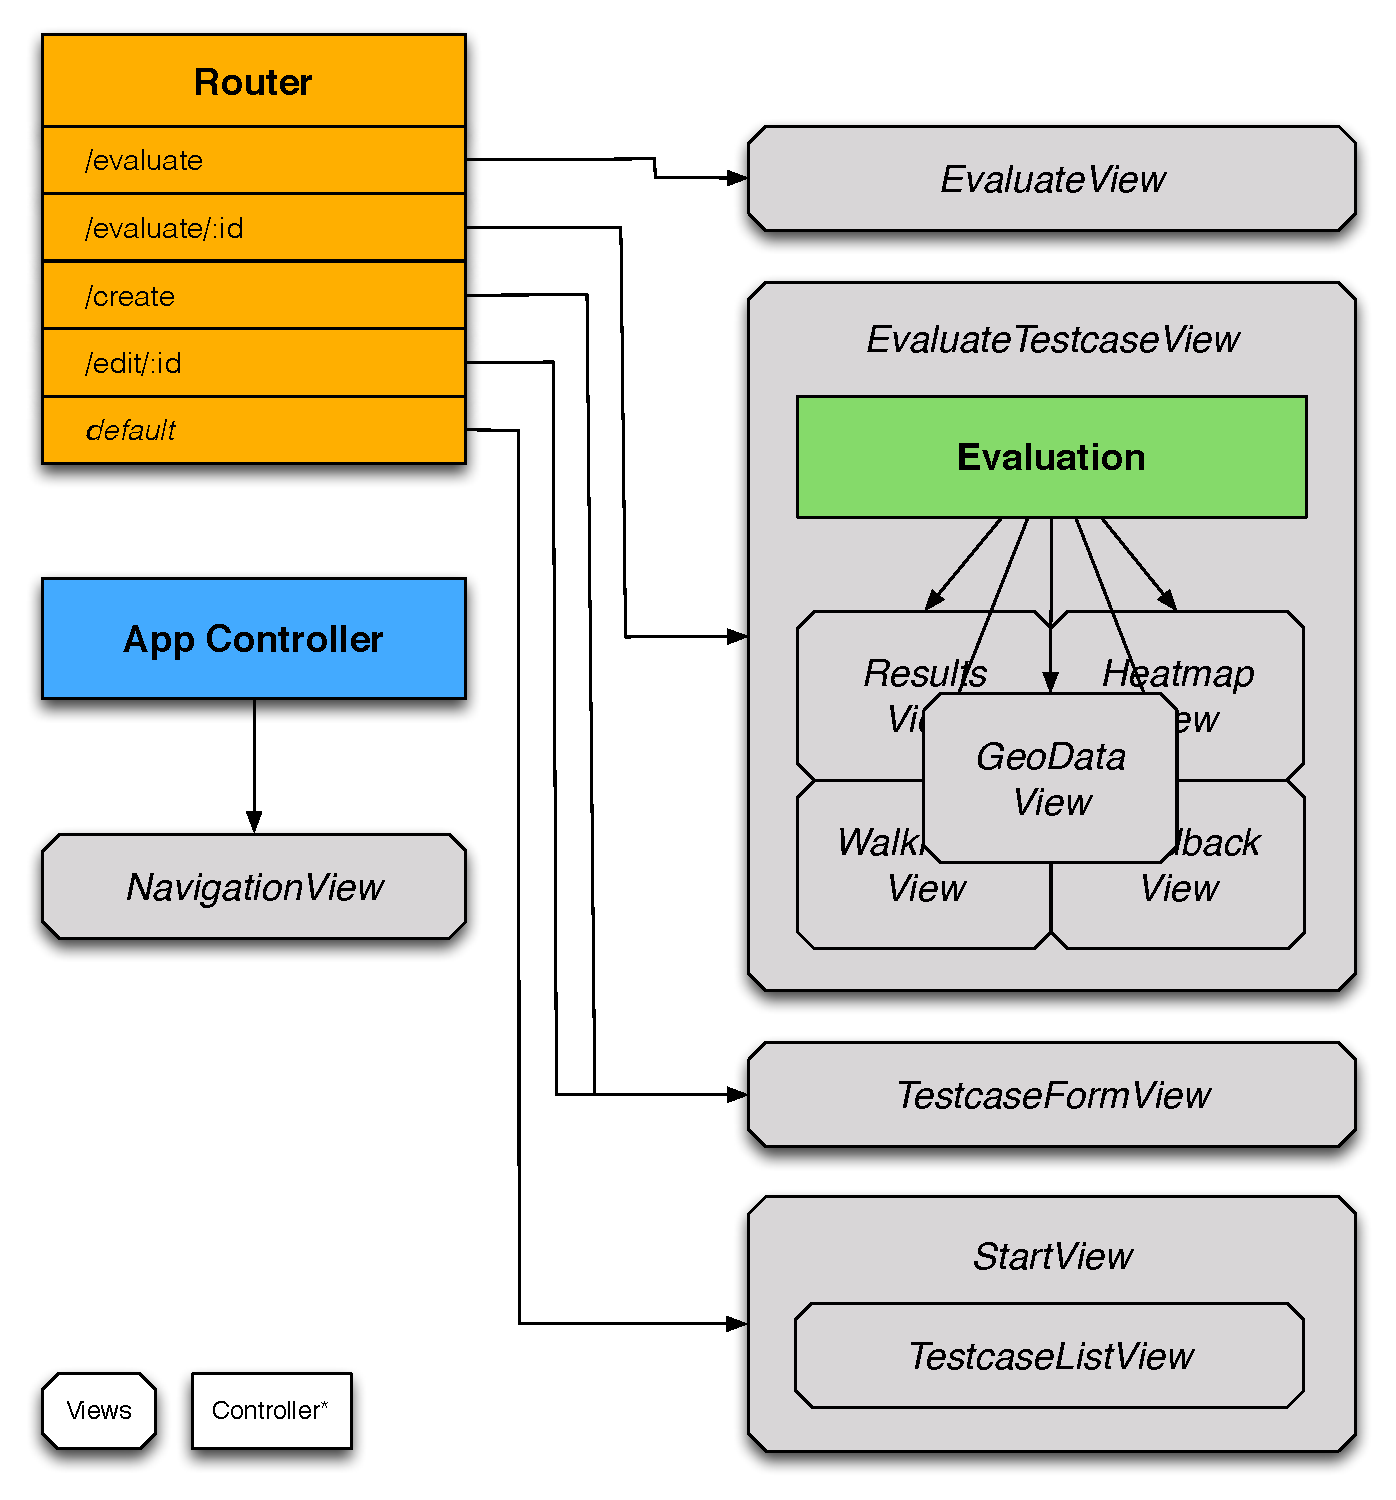
\includegraphics[scale=0.55]{./images/architecture}
\end{center}
\begin{figure}[htb]
   \centering
   \caption{Frontend Architektur der Webapplikation}
    \label{webappview}
\end{figure}

Eine weitere Komponente der Applikation sind die Datenobjekte. Backbone ermöglicht es Models zu definieren, die den Inhalt der Datenbank-Modelle widerspiegeln. Jedes Model erhält dabei eine URL, die respektiv für den Inhalt des Datenbank-Models steht. Wird das Model erzeugt, so zieht sich Backbone automatisch den Inhalt über einen Ajax-Request zur Rest-Schnittstelle. Das Gleiche geschieht bei der Persistierung. Ändert die Logik den Inhalt des Models, so kann es diesen mit der Datenbank synchronisieren über die \textit{save}-Methode. Die Nutzung von Datenobjekten in einer Backbone-Applikation verhält sich somit sehr transparent. Es scheint, als würde direkt mit den Objekten der Datenbank gearbeitet werden.\\
\\
Die Oberkategorie der Models sind \textit{Collections}. Sie beinhalten eine Menge von Models eines Typs und besitzen ebenfalls ein URL Attribut, um den Inhalt mit der Rest-Schnittstelle zu referenzieren. Anstatt eine Reihe von einzelnen Models über eine IF-Schleife zu laden, kann durch den Daten-Container ein ganzes Set einzelner Daten auf ein mal geladen werden. Dies vereinfacht die Handhabung von großen Datenreihen.\\

\subsection{Modularisierung}

Jegliche Logik in den JavaScript Dateien ist modularisiert mit RequireJS\footnote{\url{http://requirejs.org/}}. Jeder Controller oder jeder View besitzt verschiedene Dependencies, die erfüllt sein müssen, damit die Funktionen fehlerfrei ausgeführt werden können. Diese Dependencies bestehen meist aus Views, Templates oder JavaScript Bibliotheken wie jQuery. Das Objekt benötigt eine Referenz zu diesen, um mit ihnen zu arbeiten. Mit RequireJS ist es möglich, jeden Teil der Applikation zu modularisieren und sie als Dependency in anderen Modulen zu einzubinden. Ähnlich wie bei NodeJS, Java oder C geschieht dies am Kopf der Datei. Dies hilft ungemein die Struktur des Codes frei zu organisieren. Listing \ref{requirejs} wie die Modularisierung und das Einbinden von Dependencies funktioniert.

\vspace{1cm}
\begin{lstlisting}[caption=Modularisierung mit RequireJS,label=requirejs]
// Angabe der Dependencies
define([
    'jquery',
    'backbone',
    'text!templates/Start.tpl',
    'views/TestcaseListView',
    'collections/TestcaseCollection'
// Referenzierung der Dependencies zu Objekten, die innerhalb der Funktion genutzt werden koennen
], function ($, Backbone, template, TestCaseListView, TestCaseCollection) {
    var StartView = Backbone.View.extend({
        // Logik der View
        // ...
    });

    // Rueckgabewert des Moduls
    return StartView;
});
\end{lstlisting}
\vspace{0.5cm}


\subsection{Evaluation}
\label{evaluation}

Die Auswertungsmöglichkeiten der \textit{thEvaluator}-Webapplikation sind unterteilt in 5 verschiedene Widgets. Nachdem ein Testcase zur Evaluierung ausgewählt wurde, erscheint als erstes eine Übersicht mit der Gesamtanzahl der abgeschlossenen Testläufe, sowie maximal und minimal Werten der Zeit und Schritte, sowie dessen Durchschnittswert. Diese Statistiken basieren dabei auf Testläufe, die erfolgreich abgeschlossen wurden. Neben der Auflistung der meist besuchten Seiten, findet der User eine Pie-Chart über den Ausgang aller Testläufe.
\\
\begin{center}
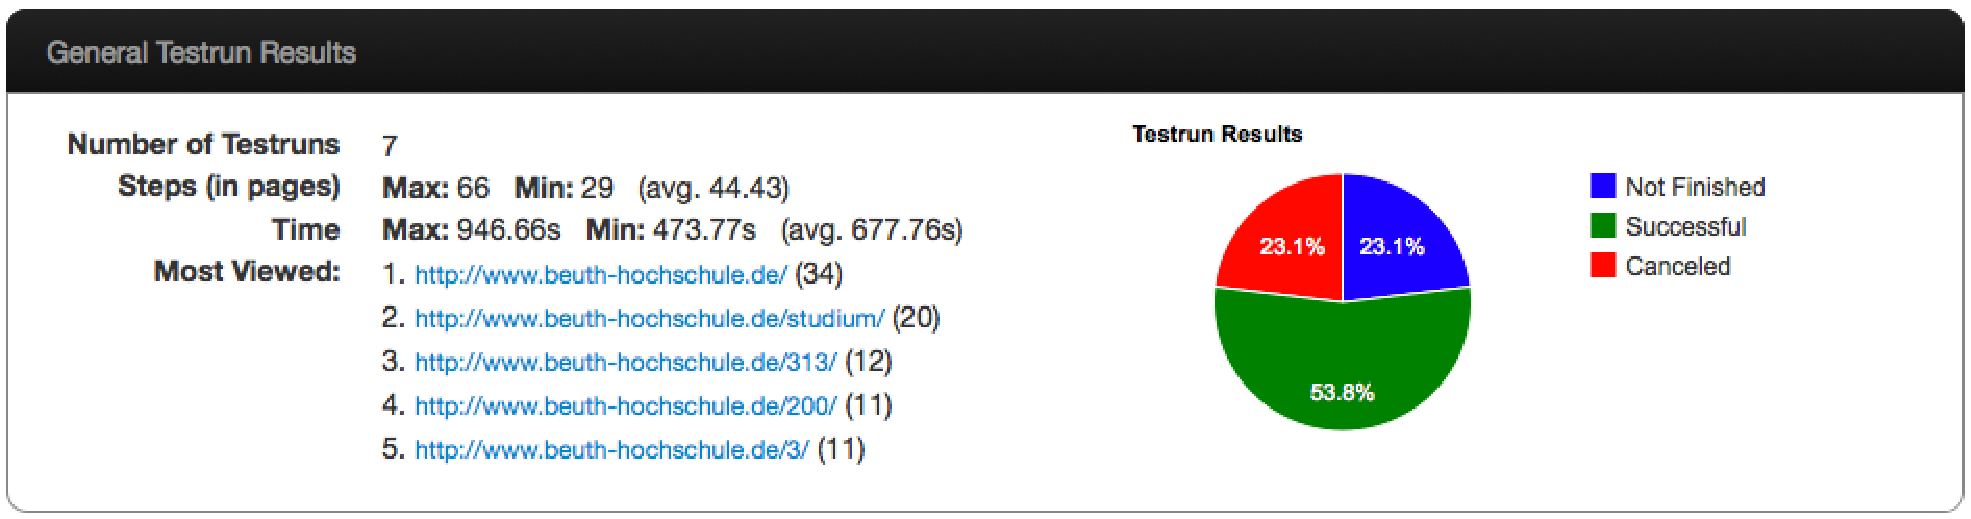
\includegraphics[scale=0.45]{./images/resultWidget}
\end{center}
\begin{figure}[htb]
   \centering
   \caption{Result-Widget}
    \label{resultWidget}
\end{figure}

Das nächste Widget ist das Maps-Widget. Es zeigt jegliche Click- und Heatmaps diverser Seiten und Testläufe, sowie dessen Gaze-Spots und Gaze-Plots. Neben der normalen Ansicht der Heatmap ist es zudem möglich, dessen Generierung in Zeitraffer mitzuverfolgen. Dadurch werden einzelne Mausbewegungen der verschiedenen User sichtbar und verfolgbar. Durch verschiedene Filter ist es möglich die Aktivität auf der ganzen Seite auf einzelne User einzuschränken. Neben der Auswahl der Seite, können Testläufe nach bestimmten Merkmalen, wie z.B. \glqq nur erfolgreiche\grqq{} oder \glqq Schnellste\grqq{}/\glqq Langsamste\grqq{}, gefiltert oder direkt einzelne Testläufe ausgewählt werden. Dadurch ist es möglich die Mausbewegung jedes einzelnen Benutzers direkt zu verfolgen und bestimmte Benutzergruppen genau zu untersuchen.\\
\\
Um die Mausposition der Seite zuordnen zu können, wird der von der Extension gespeicherte Screenshot der Seite als Hintergrund verwendet. Das Bild besitzt zwar lediglich eine Qualität von 10\% des Originals, dennoch ist gut zu erkennen, an welcher Stelle der geklickt wird. Für die Erzeugung der Heatmaps wird \textit{heatmap.js}\footnote{\url{http://www.patrick-wied.at/static/heatmapjs}} verwendet.

\begin{center}
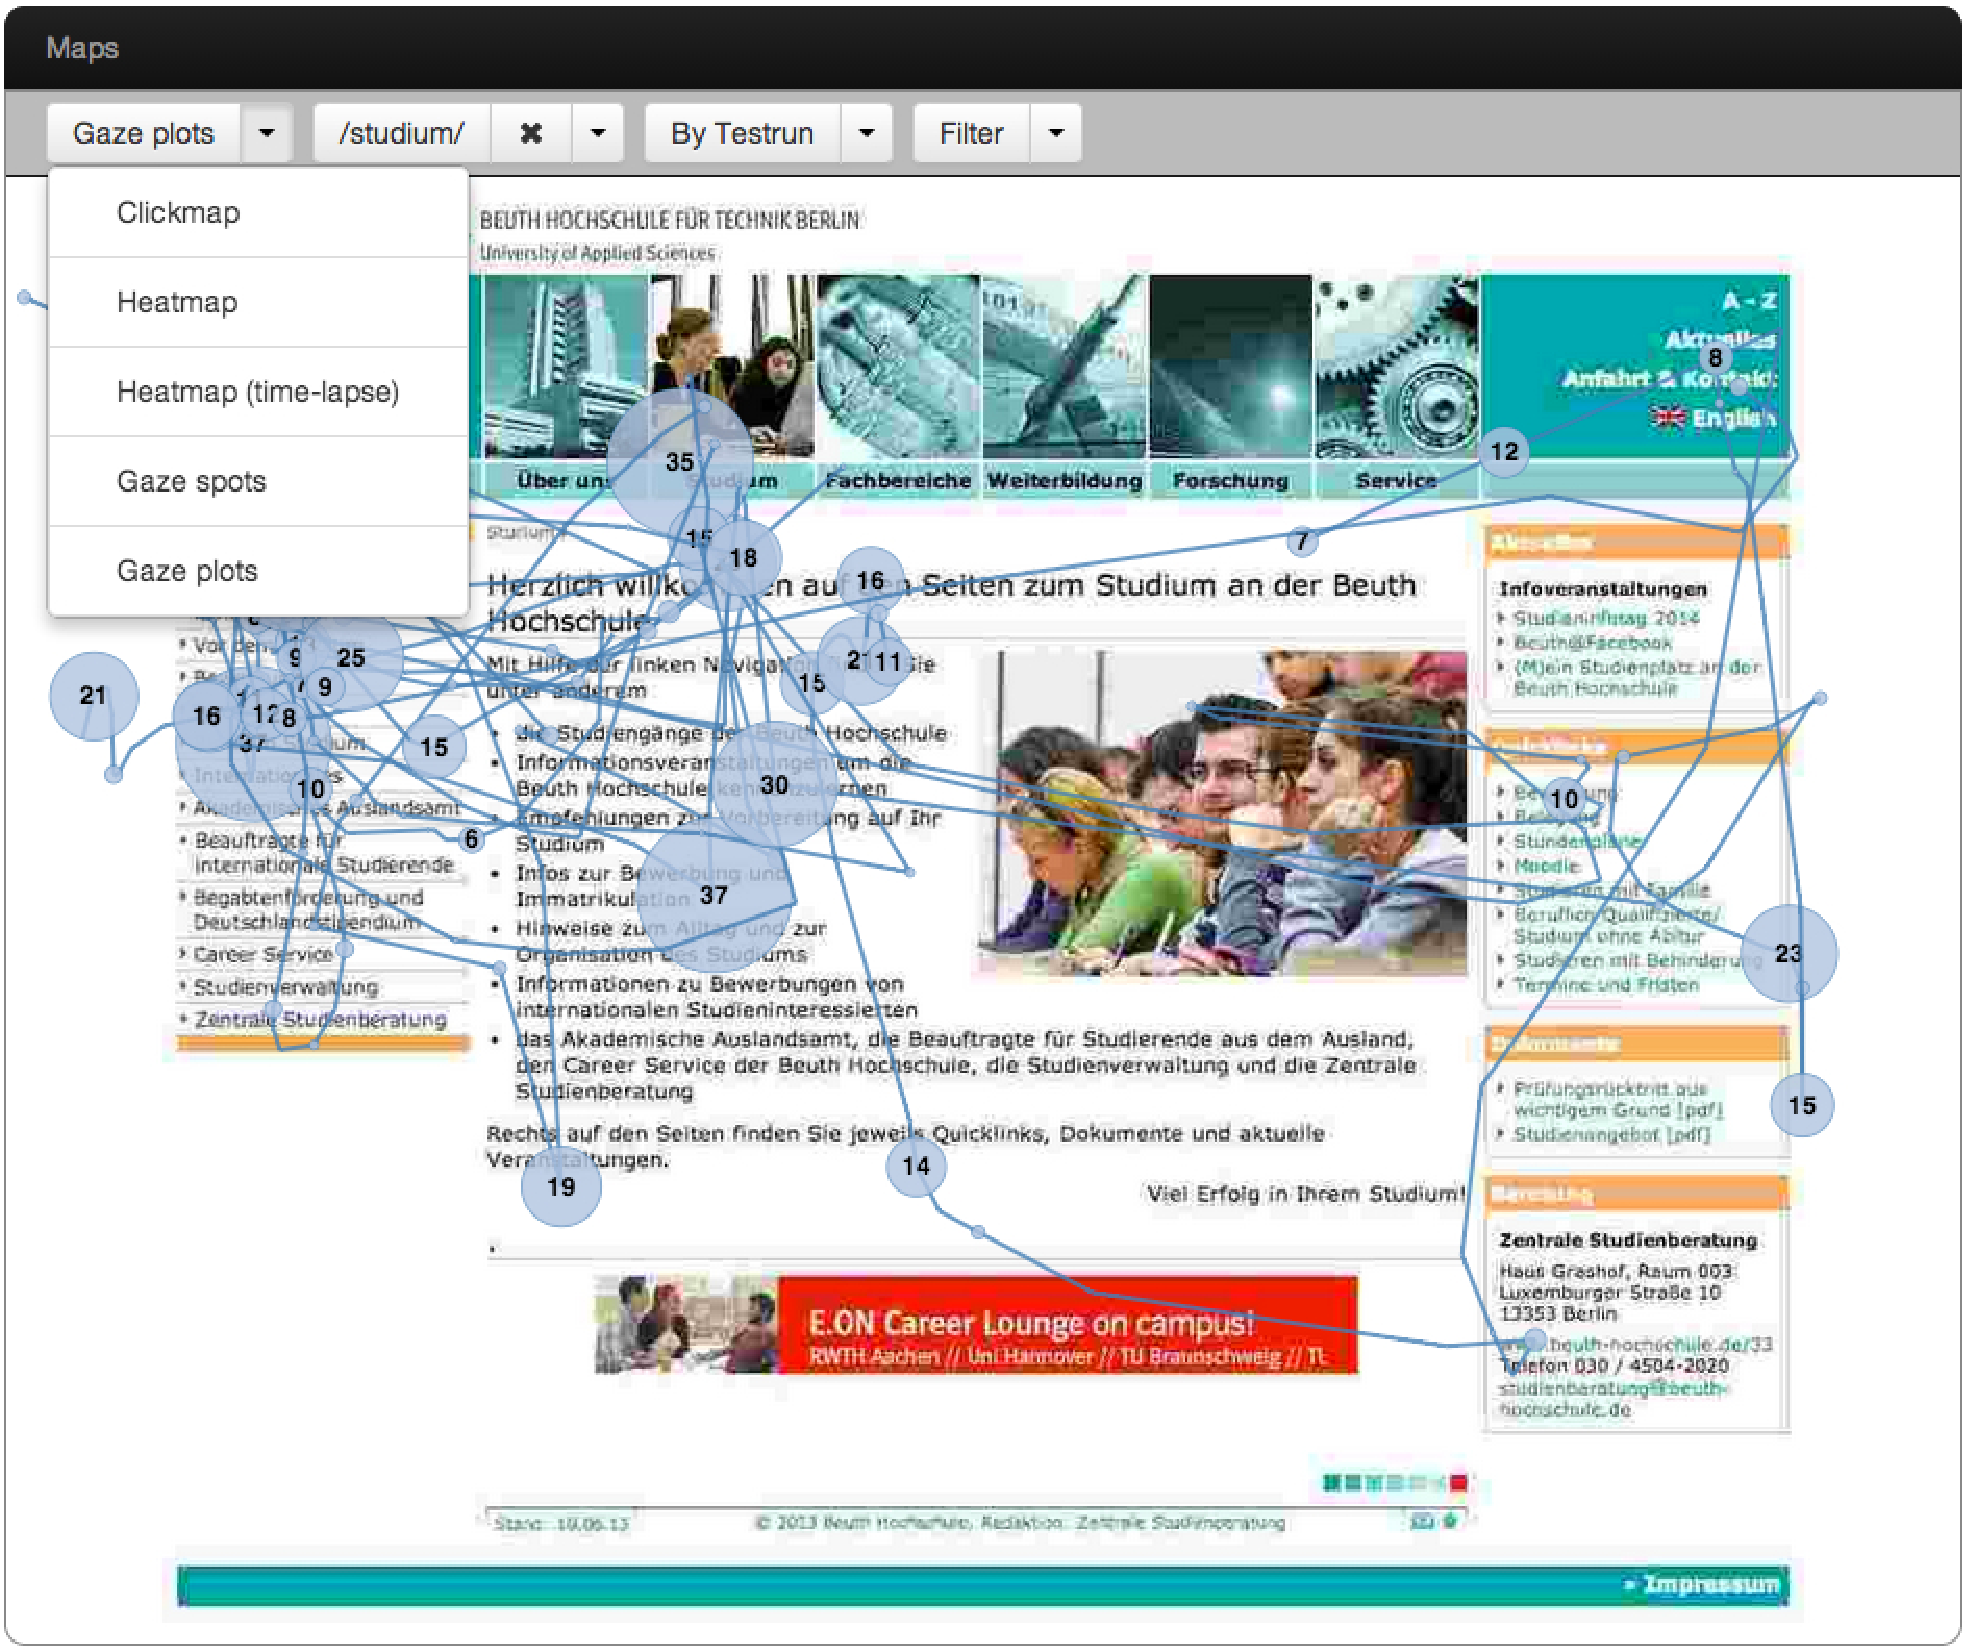
\includegraphics[scale=0.45]{./images/mapWidget}
\end{center}
\begin{figure}[htb]
   \centering
   \caption{Gaze Plot Auswertung einer Seite über das Map-Widget}
    \label{mapWidget}
\end{figure}

Da es nicht nur wichtig ist, wie sich die User auf einer einzelnen Seite verhalten, sondern auch, welchen Weg sie suchen, um an ihr Ziel zu gelangen, bietet das \textit{Walkpath}-Widget die Möglichkeit, den Verlauf des Besuches zu verfolgen. Es wird eine Art Baum aufgebaut, dessen Verzweigungen die Besucherpfade anzeigen. Die Dicke des jeweiligen Astes gibt an, wieviel Nutzer genau diesen Pfad gewählt haben. Zur Auswertung muss eine Aufgabe aus dem Testcase ausgewählt werden. Auch hier ist es wieder möglich, die Darstellung auf bestimmte Benutzergruppen einzuschränken.\\
\\
Für die Visualisierung der Daten wurde das bekannte \textit{d3}-Framework\footnote{\url{http://d3js.org/}} verwendet. Es nutzt den DOM, um mit SVG Elementen Daten zu visualisieren.

\begin{center}
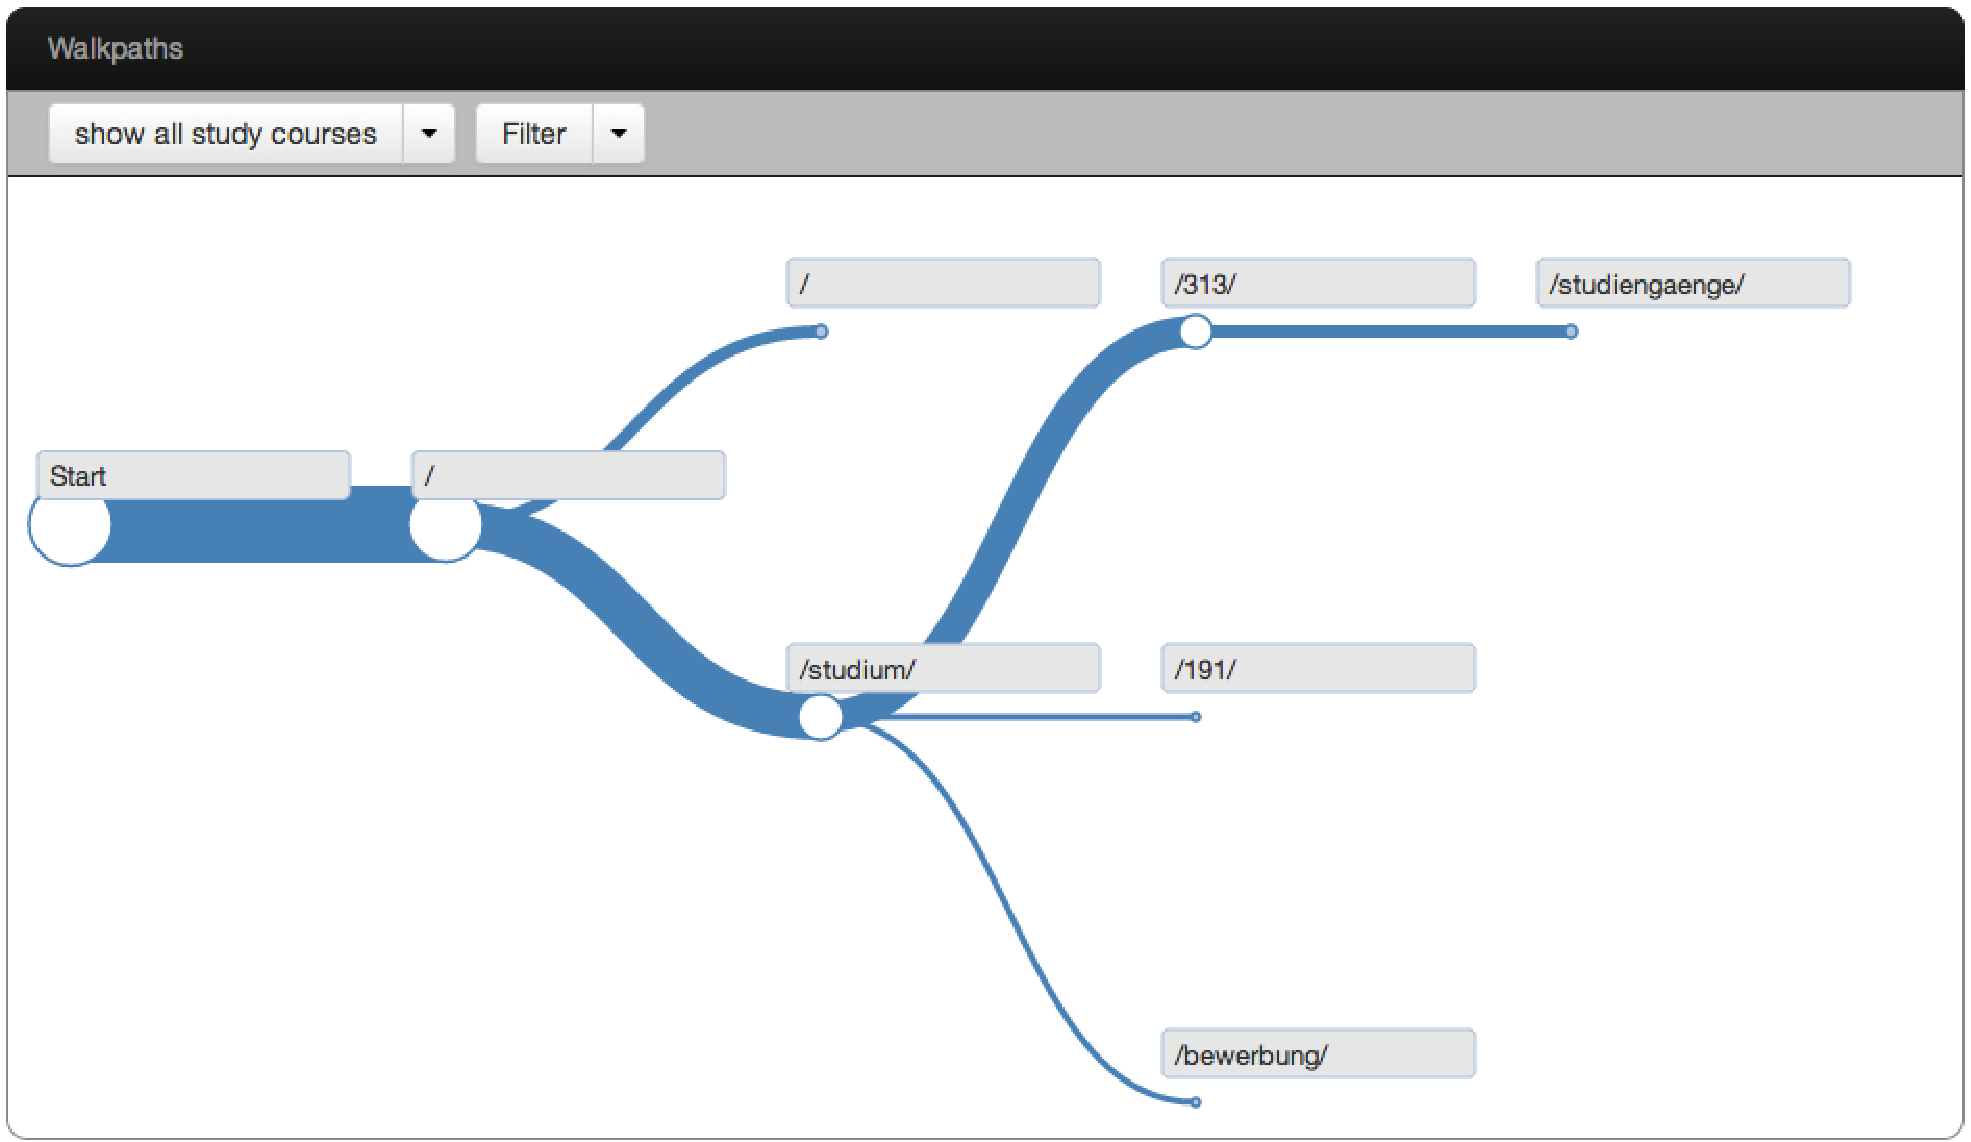
\includegraphics[scale=0.45]{./images/walkpathsWidget}
\end{center}
\begin{figure}[htb]
   \centering
   \caption{Walkpaths-Widget}
    \label{walkpathsWidget}
\end{figure}

Nachdem ein Testcase abgeschlossen ist, bekommt der User die Möglichkeit, sein persönliches Feedback abzugeben. Dem User steht eine Textbox zu Verfügung, in dem er seine Meinung entweder über den Testcase oder die Usability abgeben kann. Diese werden dann auf der Evaluation-Seite aufgelistet und können bei der Auswertung sehr hilfreiche Hinweise über spezifische Probleme bei der Benutzung der Webseite geben oder das Lösen des Testcases geben.

\begin{center}
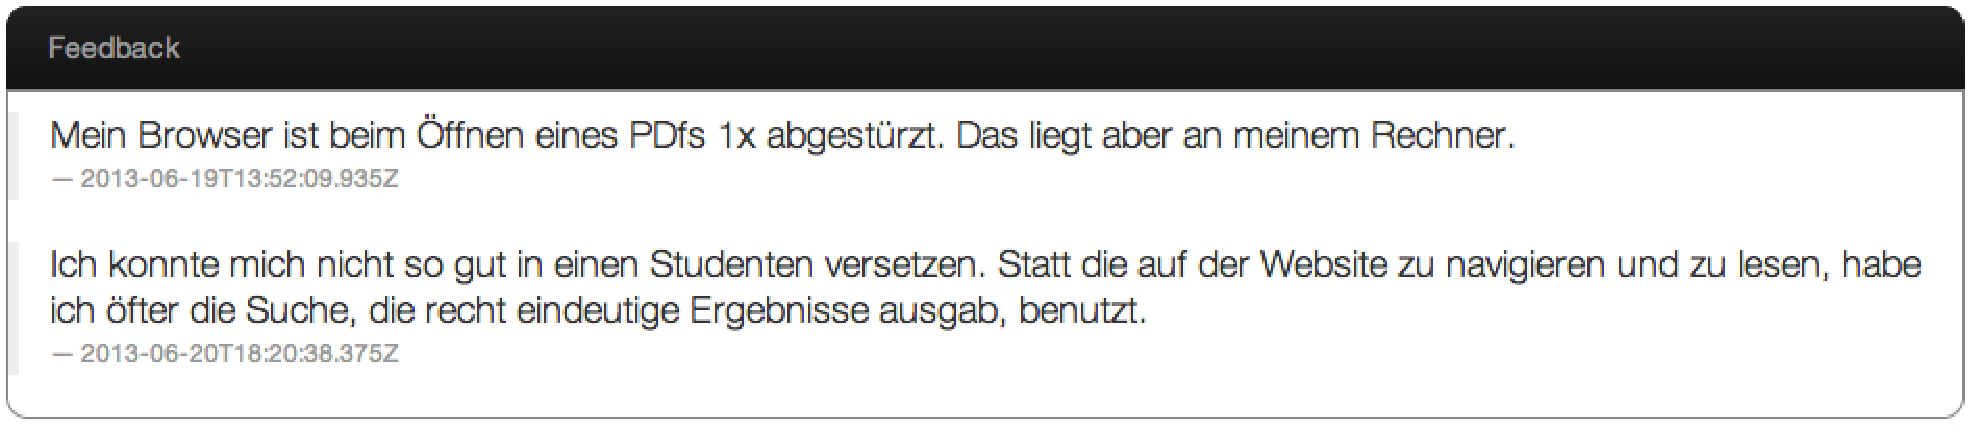
\includegraphics[scale=0.45]{./images/feedbackWidget}
\end{center}
\begin{figure}[htb]
   \centering
   \caption{Feedback-Widget}
    \label{feedbackWidget}
\end{figure}

Als letztes bietet das Geo-Widget einen Überblick über die Herkunft der Probanden. Es enthält zwar keinerlei Aussage über die Usability der Website, ermöglicht dennoch die Einsicht über die Herkunft der Probanden.

\begin{center}
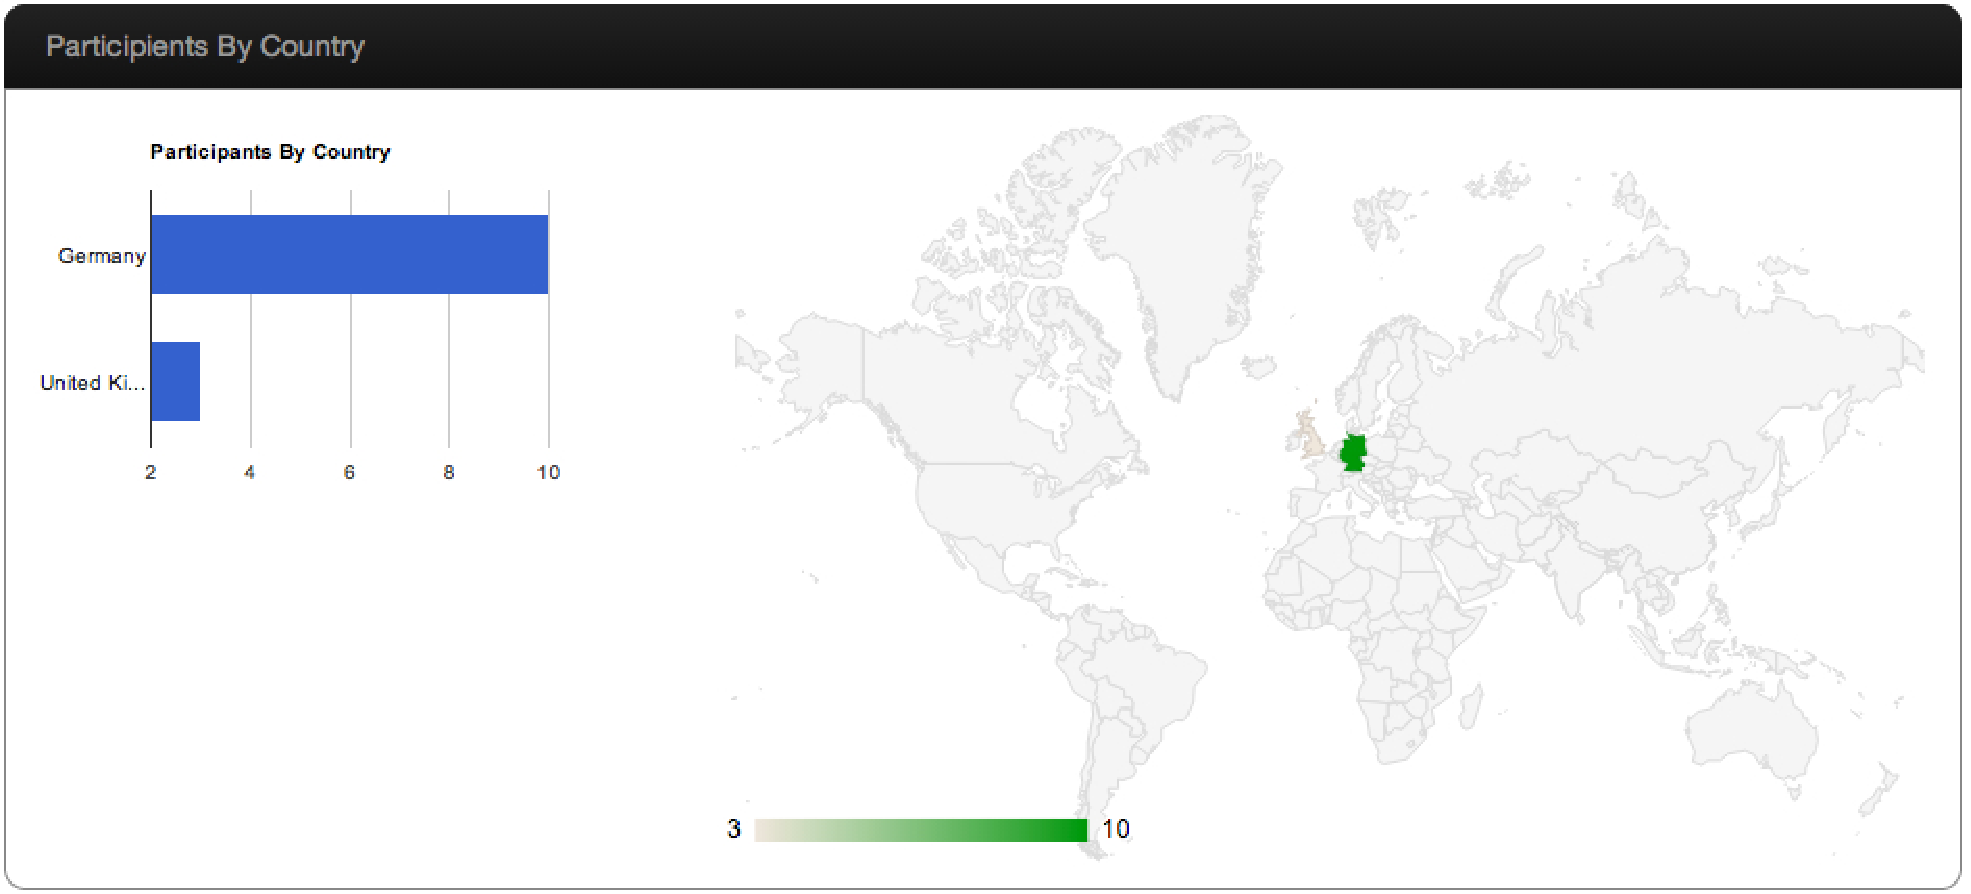
\includegraphics[scale=0.45]{./images/geoWidget}
\end{center}
\begin{figure}[htb]
   \centering
   \caption{Geo-Widget}
    \label{geoWidget}
\end{figure}